\begin{figure*}[t]
    \centering
    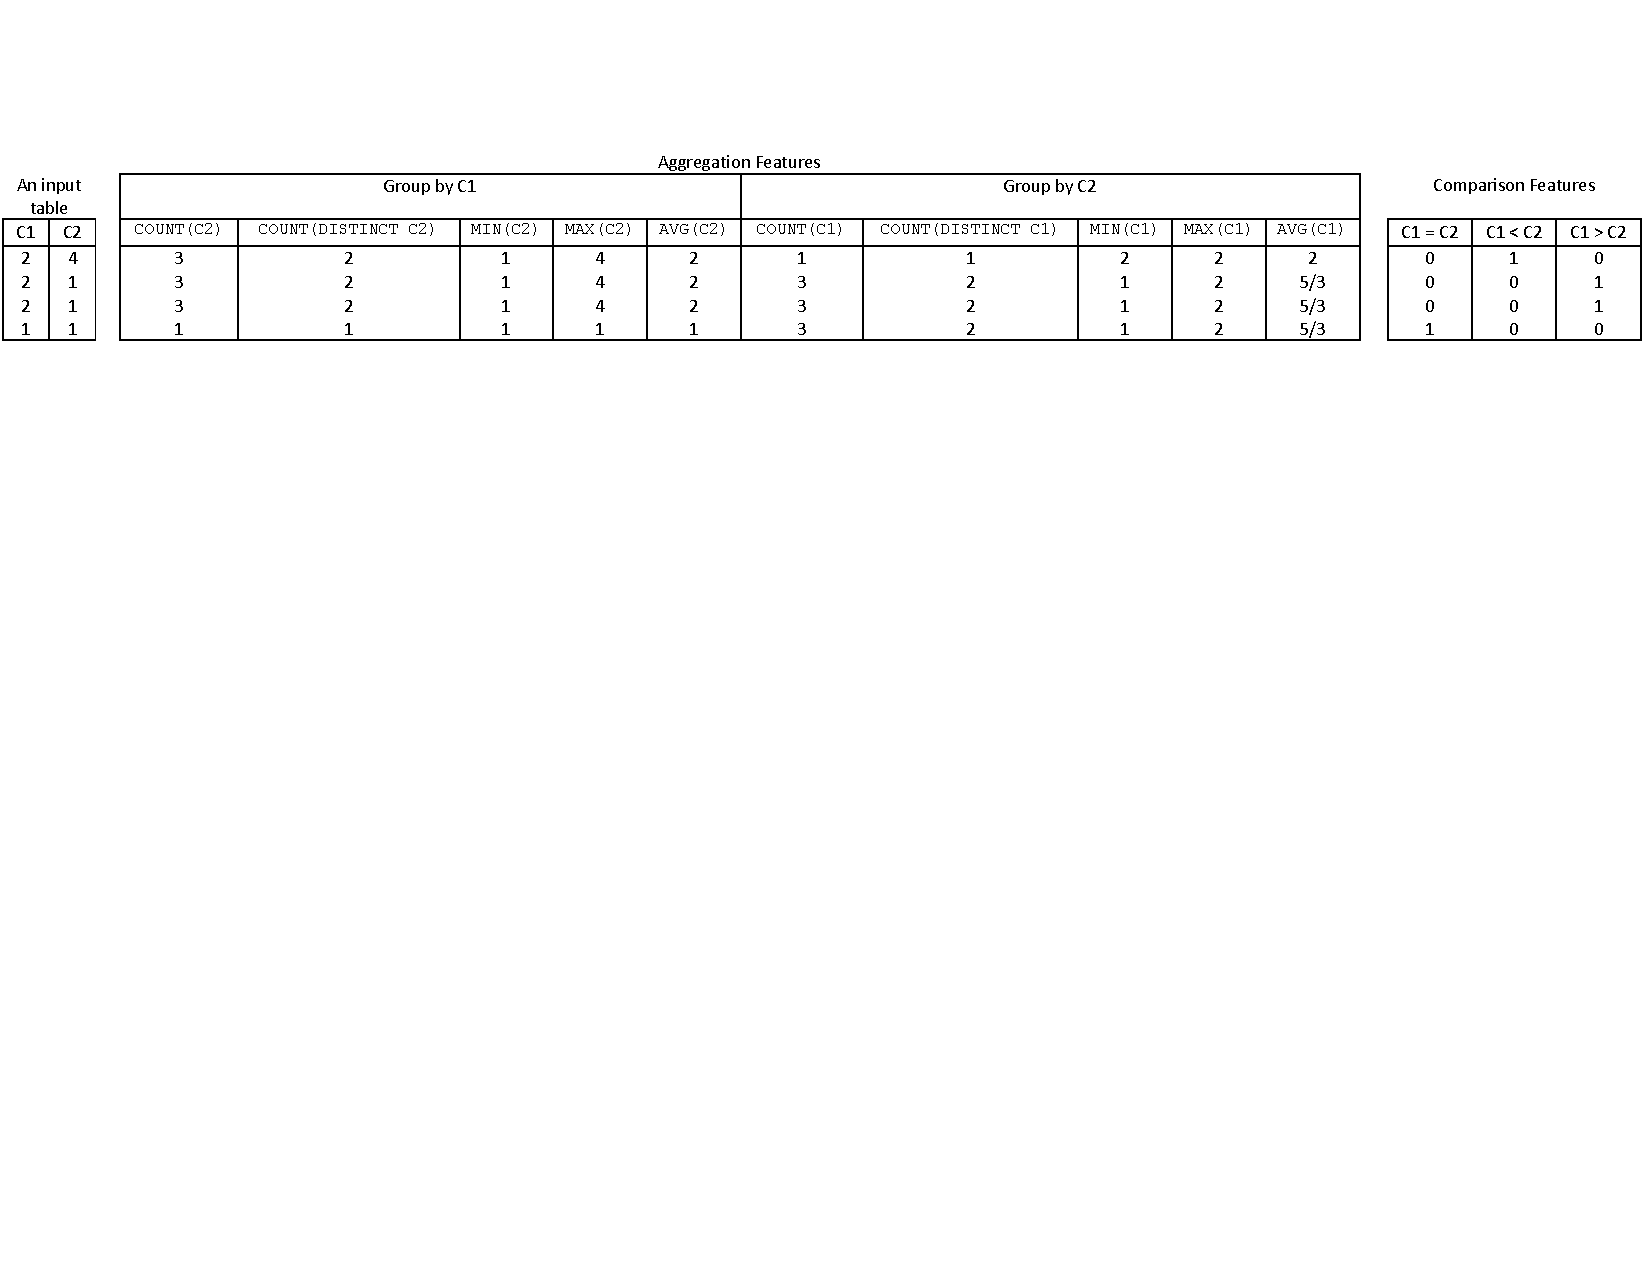
\includegraphics[scale=0.66]{featurex}
    \vspace{-7mm}
	\caption{Illustration of two new types of features
    added by \ourtool. (Left) An example input table with
    two columns: C1 and C2. (Center) The aggregation features added by
    \ourtool for the input table. (Right) The comparison features
    added by \ourtool for the input table.\newline
\strut\hspace{2mm}
    When grouping all tuples in the input table
    by column C1, there will be two
    groups: the first group includes the first 3 tuples with
    value 2 in the C1 column,
    and the second group includes the last tuple with value 1
    in the C1 column. For example, 
    the first half of the first row in the aggregation
    feature table shows the results of
    applying different aggregates
    to the first group:
    the count of C2 values is 3
    (i.e., \CodeIn{COUNT(C2)}=3); the count of
    distinct C2 values is 2 (i.e., \CodeIn{COUNT DISTINCT C2=2});
    the minimal C2 value is 1 (i.e., \CodeIn{MIN(C2)=1}),
    the maximal C2 value is 4 (i.e., \CodeIn{MAX(C2)=4}),
    the sum of C2 values is 6 (i.e., \CodeIn{SUM(C2)=6}),
    and the average C2 value is 2 (i.e., \CodeIn{AVG(C2)=2}).
   % Similar results can be computed if the table is grouped by the C2 column.
}
	\label{fig:features}
\end{figure*}
